%%%%%%%%%%%%%%%%%%%%%%%%%%%%%%%%%%%%%%%%%%%%%%%%%%%%%%%%%%%%%%%%%%%%%%%%%%%%%%%%
% ICC-12 (2026) submission -- reconciled to the accompanying ugv_uav_control
% codebase. Scope (proven offline / implemented / simulation / future) is stated
% in prose; see Sec. VI (Theoretical Properties) and the Sec. VII scope paragraph.
%%%%%%%%%%%%%%%%%%%%%%%%%%%%%%%%%%%%%%%%%%%%%%%%%%%%%%%%%%%%%%%%%%%%%%%%%%%%%%%%

\documentclass[letterpaper, 10 pt, conference]{ieeeconf}  % Comment this line out if you need a4paper

%\documentclass[a4paper, 10pt, conference]{ieeeconf}      % Use this line for a4 paper
\usepackage{amsmath}
\usepackage{amssymb}
\usepackage{graphicx}
\usepackage{censor}
\usepackage{comment}
\usepackage{multirow}
\usepackage{booktabs}
\usepackage{url}
% Figures live beside this .tex (self-contained); resolve locally and on Overleaf
% when the figure files are uploaded flat to the project root (bare filenames).
\graphicspath{{./}}
\usepackage{tikz}
\usetikzlibrary{arrows.meta,positioning,calc,fit,backgrounds}

\IEEEoverridecommandlockouts                              % This command is only needed if
                                                          % you want to use the \thanks command

\overrideIEEEmargins                                      % Needed to meet printer requirements.

\DeclareMathOperator{\tr}{tr}
\newcommand{\Rset}{\mathbb{R}}

% Compact bibliography spacing (content-preserving; recovers a few lines for the page budget)
\let\oldthebibliography\thebibliography
\renewcommand{\thebibliography}[1]{%
  \oldthebibliography{#1}%
  \setlength{\itemsep}{0pt}%
  \setlength{\parsep}{0pt}%
  \setlength{\topsep}{0pt}%
}
% Tighten spacing around the (many) floats -- content-preserving page tightening
\setlength{\textfloatsep}{10pt plus 2pt minus 2pt}
\setlength{\floatsep}{8pt plus 2pt minus 2pt}
\setlength{\intextsep}{10pt plus 2pt minus 2pt}

% ---- results macros. STEADY-STATE window t>=8s (skips takeoff/EKF-convergence transient).
% Fixed-system co-design numbers (C1 continuous vs C2 event-triggered, track2, headless, R=3).
% All values regenerated after the /cmd_vel-collision fix, so the UAV is genuinely controlled.
\newcommand{\RESsolvesCone}{\ensuremath{797\pm16}}\newcommand{\RESsolvesCthree}{\ensuremath{32\pm1}}
\newcommand{\RESmsCone}{\ensuremath{3.9\pm0.1}}\newcommand{\RESmsCthree}{\ensuremath{7.9\pm0.4}}
\newcommand{\REScpuCone}{\ensuremath{3123\pm56}}\newcommand{\REScpuCthree}{\ensuremath{253\pm6}}
\newcommand{\RESoffCone}{\ensuremath{0.128\pm0.002}}\newcommand{\RESoffCthree}{\ensuremath{0.060\pm0.005}}
\newcommand{\REScov}{\ensuremath{0.0095}}\newcommand{\RESsolveRed}{25}\newcommand{\REScpuRed}{12}
% reproducibility: identical-config UGV ground-truth path fork
\newcommand{\RESforkGUI}{2.7}\newcommand{\RESforkHL}{0.03}
% Altitude-policy comparison (hairpin, headless, GSD noise, R=3): adaptive vs fixed-low(2.5) vs fixed-high(7).
% mean/max estimation covariance tr(Sigma); each fixed policy is dominated on one axis.
\newcommand{\RESaltAdaptMean}{\ensuremath{0.0065}}\newcommand{\RESaltLowMean}{\ensuremath{0.0062}}\newcommand{\RESaltHiMean}{\ensuremath{0.0105}}
\newcommand{\RESaltAdaptMax}{\ensuremath{0.016}}\newcommand{\RESaltLowMax}{\ensuremath{0.14}}\newcommand{\RESaltHiMax}{\ensuremath{0.030}}
\newcommand{\RESaltHiPen}{61}\newcommand{\RESaltLowRatio}{9}
\newcommand{\RESaltLo}{2.5}\newcommand{\RESaltHiZ}{5.1}

\title{\LARGE \bf
Perception-Constrained Altitude Control for Aerial--Ground \\
Cooperative Tracking with a Shared Downward Camera
}

\author{\censor{Shlok Mehndiratta, Divyam Sood, Prashant Gupta, and Arijit Sen}%
\thanks{The authors are with the Indian Institute of Science Education and
Research (IISER) Bhopal, India.
\censor{
{\tt\small \{shlokm23, divyam23, prashant23\}@iiserb.ac.in},
{\tt\small ajsen@iiserb.ac.in}}%
}
}


\begin{document}



\maketitle
\thispagestyle{empty}
\pagestyle{empty}


%%%%%%%%%%%%%%%%%%%%%%%%%%%%%%%%%%%%%%%%%%%%%%%%%%%%%%%%%%%%%%%%%%%%%%%%%%%%%%%%
\begin{abstract}
We present a reproducible software-in-the-loop (SITL) study of
aerial--ground cooperative tracking in which a single downward UAV camera is the ground
vehicle's {sole} exteroceptive sensor, serving simultaneously as its navigation
reference (path segmentation) and its state estimator (ArUco/EKF). This shared-sensor architecture couples navigation and estimation through a single control variable - the UAV
altitude - and this coupling is the organizing principle of our design: low altitude sharpens estimation (ground-sampling noise $R\propto z^2$) but starves navigation coverage (the path
lookahead leaves the camera footprint), while high altitude does the reverse. We develop a perception-constrained altitude policy guided by the shared-camera coverage constraint and {demonstrate it closed-loop in SITL}. 
\end{abstract}


%%%%%%%%%%%%%%%%%%%%%%%%%%%%%%%%%%%%%%%%%%%%%%%%%%%%%%%%%%%%%%%%%%%%%%%%%%%%%%%%
\section{INTRODUCTION}

The deployment of Unmanned Ground Vehicles (UGVs) in unstructured or GPS-denied environments is heavily constrained by their limited perception horizons. Onboard sensors such as LiDAR and stereo cameras have been used in such vehicles for navigation purposes, but they suffer from occlusion,
narrow fields of view (FoV), and an inability to anticipate the upcoming path. To mitigate this, aerial--ground cooperative systems employ anUnmanned Aerial Vehicle (UAV) as an elevated ``eye in the sky'' for a
perception-limited UGV.

Most cooperative-tracking frameworks treat the UAV as a {passive} observer:
it follows a predefined trajectory or simply minimizes distance to the UGV,
treating the UGV's state estimation as a downstream byproduct
\cite{mayne2000constrained}. This decoupling is fragile: when the UGV maneuvers
aggressively or is occluded, the UAV can lose the target, the estimation
covariance grows, and tracking degrades. Active-perception planning, where the
sensor trajectory is optimized to maximize information gain
\cite{falanga2018pampc}, addresses part of this but typically relies on
continuous, computationally expensive replanning and rarely integrates robust
tracking guarantees for the aerial vehicle.

We present a shared-camera perception-control architecture in
which {both} vehicles adapt to the ground vehicle's estimation uncertainty.
Its contributions, as realized in the accompanying open implementation, are:

\begin{itemize}
\item  {A perception-constrained altitude policy, formalized and demonstrated
closed-loop.} With one downward camera serving both the ground vehicle's navigation (path
segmentation) and its state estimate (ArUco/EKF) \cite{platt2010belief,vandenberg2012motion},
low altitude sharpens estimation ($R\propto z^2$) but starves navigation coverage; the policy
flies as low as segmentation allows and climbs into turns. 

\item  We show a perception-driven event trigger cuts the UAV nominal (aerial) planner's online re-solves $\approx\!\RESsolveRed\times$ ($\RESsolvesCone\!\to\!\RESsolvesCthree$ per run) and its CPU $\approx\!\REScpuRed\times$ at matched estimation quality (covariance $\REScov$, $\approx\!99.9\%$ visibility for both continuous and event-triggered planning).

\item  {A reproducible SITL realization} in ROS\,2/Gazebo
(vision/ArUco pipeline, view-quality-coupled EKF, belief-space UGV MPC, and the UAV
planner/ancillary pair \cite{mayne2005robust,eqtami2010event}). Code and data are openly
available.\footnote{\url{https://github.com/shlok-mehndiratta/ugv_uav_control}}
\end{itemize}
The remainder of the paper is organized as follows. Section~\ref{sec:related} reviews related
work; Section~\ref{sec:problem} states the problem; Section~\ref{sec:arch} gives
the vehicle and perception models; Section~\ref{sec:method} develops the coupled
event-triggered MPC; Section~\ref{sec:theory} states the theoretical
properties and the exact implementation status; and Section~\ref{sec:results}
reports the simulation study.

\section{RELATED WORK}
\label{sec:related}

 Tube MPC \cite{mayne2005robust,langson2004tubes,chisci2001persistent}
decomposes control into a nominal plan and an ancillary law that confines the true state to a
robust positively invariant (RPI) tube; Rakovi\'c et al. \cite{mRPI} give the standard
outer approximation of the minimal RPI set, and the nonlinear case is treated in
\cite{mayne2011tube}. These guarantees assume a fixed, bounded disturbance set and constraint
tightening computed offline. Time-varying (homothetic/parameterized) tubes generalize the
fixed tube but require the scaling to enter the optimization with its own feasibility argument;
our online adaptivity (Section~\ref{sec:method}) is a lighter-weight surrogate.

 Perception-aware trajectory optimization for
quadrotors \cite{falanga2018pampc,spasojevic2020perception} and active visual localization
\cite{zhang2019fisher} shape motion to serve estimation. Belief-space planning
\cite{platt2010belief,vandenberg2012motion,prentice2009belief,indelman2015planning} augments
the planning state with the estimator covariance helping planning under partial
observability \cite{kaelbling1998planning} and of active SLAM \cite{cadena2016past,placed2023survey}.
Our belief-space UGV controller is in this family. Our architecture is
{bidirectional}: the {target} shapes its trajectory to stay observable while the
{tracker} adapts both its altitude and its robustness margin to perception quality.

 {Cooperative aerial--ground teams.} Using an aerial vehicle as an ``eye in the sky'' for
a ground robot has been demonstrated \cite{grocholsky2006cooperative}, including recent
perception-limited-UGV navigation \cite{li2024colag} and aerial-vision guidance of a
perception-less ground vehicle \cite{santos2024aerial}, alongside quadrotor target-tracking
under field-of-view and occlusion constraints \cite{thomas2017autonomous,penin2018vision} and
EKF-based cooperative localization \cite{roumeliotis2002distributed,kia2016cooperative}. These
systems typically fix the aerial vehicle's altitude and treat it as a passive relay; we show
instead that altitude is an active perception control input whose optimal use is dictated by
the shared-camera coupling.

 vent-triggered and self-triggered control
\cite{tabuada2007event,heemels2012introduction} re-solve only when a state-dependent condition
fires, and extend to robust MPC of nonlinear systems \cite{eqtami2010event,li2014event}. We
instantiate a perception-driven trigger with a critical tube-exit condition plus anticipatory
conditions.

\section{PROBLEM FORMULATION}
\label{sec:problem}

A UAV tracks a UGV in a global frame $\mathcal{F}_W$. The UAV carries the only
exteroceptive sensor: a downward monocular camera that detects an ArUco marker on
the UGV, yielding a noisy pose measurement whose quality depends on the imaging
geometry. An EKF fuses these detections with UGV wheel odometry to produce a
belief $(\mu,\Sigma)$ over the UGV state. The objective is to (i) keep the UGV
inside the camera footprint so that $\Sigma$ stays bounded, (ii) track the UGV
robustly under bounded disturbances, and (iii) do so while limiting the number of
online optimizations. The UGV must track a ground lane while remaining
observable.

\section{System Architecture and Models}
\label{sec:arch}

Fig.~\ref{fig:system} shows the implemented system and its signal flow.

\begin{figure}[t]
\centering
\resizebox{0.99\columnwidth}{!}{%
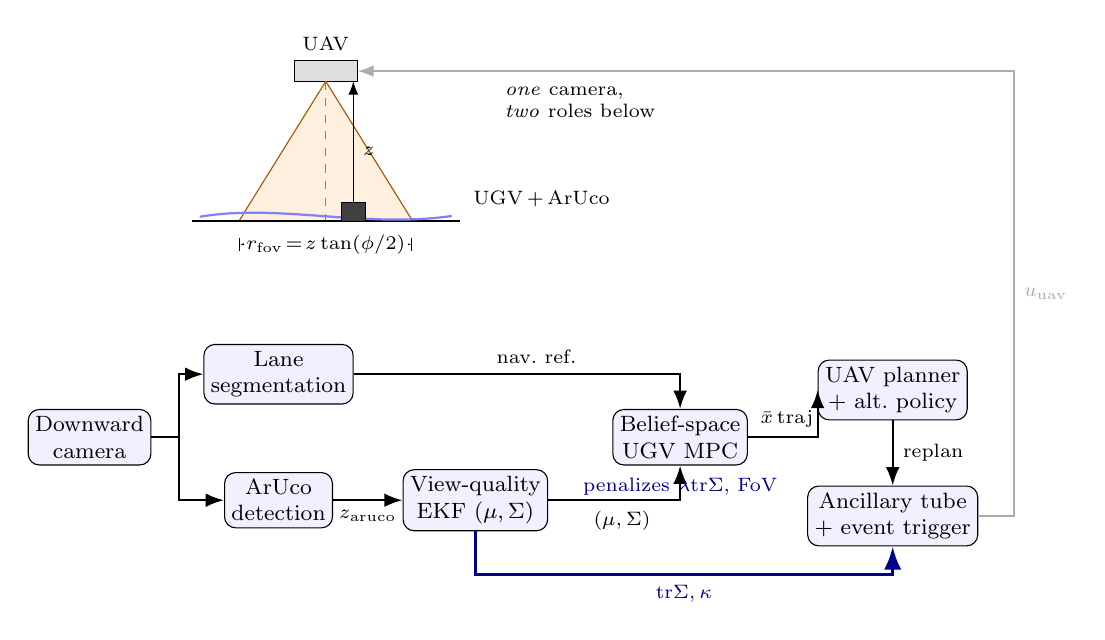
\begin{tikzpicture}[font=\footnotesize,>=Latex,
  blk/.style={draw,rounded corners,align=center,minimum height=6.5mm,inner sep=2.5pt,fill=blue!6},
  sig/.style={->,thick},
  cpl/.style={->,very thick,blue!55!black},
  fb/.style={->,semithick,gray!65}]

% ================= physical geometry (top strip) =================
\begin{scope}[shift={(0,0.2)}]
  \node[draw,fill=gray!25,minimum width=8mm,minimum height=2.6mm] (uav) at (3.0,1.9) {};
  \node[font=\scriptsize] at (3.0,2.25) {UAV};
  \coordinate (cam) at (3.0,1.77);
  \fill[orange!12] (cam) -- (1.9,0) -- (4.1,0) -- cycle;
  \draw[orange!65!black] (cam)--(1.9,0); \draw[orange!65!black] (cam)--(4.1,0);
  \draw[dashed,gray] (cam)--(3.0,0);
  \draw[<->] (3.35,0)--(3.35,1.77) node[midway,right=0pt,font=\scriptsize]{$z$};
  \draw[thick] (1.3,0)--(4.7,0);
  \draw[thick,blue!50] (1.4,0.05) .. controls (2.4,0.22) and (3.5,-0.10) .. (4.6,0.06);
  \node[draw,fill=black!75,minimum width=3mm,minimum height=1.8mm] (ugvp) at (3.35,0.11) {};
  \node[font=\scriptsize,anchor=west] at (4.75,0.28) {UGV\,+\,ArUco};
  \draw[|<->|] (1.9,-0.30)--(4.1,-0.30) node[midway,fill=white,inner sep=1pt,font=\scriptsize]{$r_{\mathrm{fov}}\!=\!z\tan(\phi/2)$};
  \node[align=left,font=\scriptsize,anchor=west] at (5.15,1.5) {\textit{one} camera,\\ \textit{two} roles below};
\end{scope}

% ================= dataflow (bottom), left-to-right =================
\node[blk] (cam2)   at (0.0,-2.55) {Downward\\camera};
\node[blk] (seg)    at (2.4,-1.75) {Lane\\segmentation};
\node[blk] (aruco)  at (2.4,-3.35) {ArUco\\detection};
\node[blk] (ekf)    at (4.9,-3.35) {View-quality\\EKF $(\mu,\Sigma)$};
\node[blk] (ugvmpc) at (7.5,-2.55) {Belief-space\\UGV MPC};
\node[blk] (plan)   at (10.2,-1.95) {UAV planner\\+ alt.\ policy};
\node[blk] (anc)    at (10.2,-3.55) {Ancillary tube\\+ event trigger};

% one camera image -> two roles
\draw[sig] (cam2.east) -- ++(0.35,0) |- (seg.west);
\draw[sig] (cam2.east) -- ++(0.35,0) |- (aruco.west);
% navigation role
\draw[sig] (seg.east) -| node[pos=0.28,above,font=\scriptsize]{nav.\ ref.} (ugvmpc.north);
% estimation role
\draw[sig] (aruco.east) -- node[below,font=\scriptsize]{$z_{\mathrm{aruco}}$} (ekf.west);
\draw[sig] (ekf.east) -| node[pos=0.28,below,font=\scriptsize]{$(\mu,\Sigma)$} (ugvmpc.south);
% controllers
\draw[sig] (ugvmpc.east) -| node[pos=0.28,above,font=\scriptsize]{$\bar x$\,traj} (plan.west);
\draw[sig] (plan.south) -- node[right,font=\scriptsize]{replan} (anc.north);
% coupling: EKF (trSigma, kappa) -> event trigger
\draw[cpl] (ekf.south) -- ++(0,-0.55) -| node[pos=0.25,below,font=\scriptsize]{$\mathrm{tr}\Sigma,\kappa$} (anc.south);
% feedback: ancillary command -> UAV (closes loop, sets camera pose)
\draw[fb] (anc.east) -- ++(0.45,0) |- node[pos=0.25,right,font=\scriptsize]{$u_{\mathrm{uav}}$} (uav.east);
\node[blue!55!black,font=\scriptsize,align=center,below=1pt of ugvmpc]{penalizes $\lambda\mathrm{tr}\Sigma$, FoV};
\end{tikzpicture}}
\caption{System overview. {Top:} the physical geometry --- a downward-camera UAV at
altitude $z$ views an ArUco-tagged UGV on a curving lane within a footprint of radius
$r_{\mathrm{fov}}=z\tan(\phi/2)$. {Bottom:} the single camera image feeds {two}
roles: lane segmentation provides the UGV's navigation reference, and ArUco detection feeds the
view-quality EKF $(\mu,\Sigma)$; both drive the belief-space UGV MPC (which penalizes
$\lambda\,\mathrm{tr}\Sigma$ and FoV exit), whose predicted trajectory the UAV planner tracks
under the perception-constrained altitude policy, executed by the ancillary tube/event-trigger
controller ( {blue:} the EKF covariance and curvature drive the event trigger). This
dual role of one sensor is the coverage--resolution coupling studied in the paper.}
\label{fig:system}
\end{figure}

\subsection{UGV dynamics}
The UGV uses unicycle kinematics with first-order actuator lag. Let
$\mathbf{x}_g = [x_g, y_g, \theta, v, \omega]^T$ be the state, $(x_g,y_g)$ the
position, $\theta$ the heading, $(v,\omega)$ the linear/angular velocities, and
$\mathbf{u}_g = [v_c, \omega_c]^T$ the commanded velocities. The discrete-time
dynamics are
\begin{equation}
\mathbf{x}_{g,k+1} = \mathbf{f}_g(\mathbf{x}_{g,k}, \mathbf{u}_{g,k}) + \mathbf{w}_g,
\end{equation}
where the actuator lag is governed by time constants $\tau_v,\tau_\omega$ and
$\mathbf{w}_g$ is process noise.

\subsection{UAV model}
Although the platform is a quadrotor, the planner and the ancillary tracker treat
it as a  {velocity-controlled point mass} (single integrator); an
inner-loop attitude/thrust controller, provided by the Gazebo velocity-control
plugin, is assumed to realize commanded velocities. With position
$\mathbf{p}=[p_x,p_y,p_z]^T$ and velocity command $\mathbf{u}=[v_x,v_y,v_z]^T$,
\begin{equation}
\mathbf{p}_{k+1} = \mathbf{p}_k + \Delta t\, \mathbf{u}_k + \mathbf{w}_k,
\qquad A_d=I_3,\ B_d=\Delta t\, I_3,
\label{eq:uav_disc}
\end{equation}
with bounded disturbance $\mathbf{w}_k\in\mathbb{W}$. All three axes are fully
actuated: $v_z$ is a genuine decision variable and the altitude policy of
Sec.~\ref{sec:coverage} is realized closed-loop in SITL (the UAV altitude spans
$[2.5,7]$\,m; Sec.~\ref{sec:results}).




\subsection{Ground-sampling-distance measurement model}

The accuracy of visual localization depends on the camera's ground sampling distance (GSD), which increases linearly with UAV altitude. Assuming the image-space localization error remains approximately constant in pixels, the corresponding metric position error grows proportionally to the GSD, implying that the position-measurement covariance scales quadratically with altitude. Let $z$ denote the UAV altitude, $z_0$ a reference altitude, $d=\|\mathbf{p}^{xy}-\mathbf{p}_g\|$ the horizontal UAV--UGV separation, and $r_{\mathrm{fov}}(z)=z\tan(\phi/2)$ the camera footprint radius. The measurement covariance is modeled as
\begin{equation}
R(z)=R_0\left(\frac{z}{z_0}\right)^2
\left(1+\left(\frac{d}{r_{\mathrm{fov}}}\right)^2\right),
\label{eq:Rgsd}
\end{equation}
where $R_0$ is the baseline ArUco measurement covariance at the reference altitude $z_0$. The second term provides a mild inflation of the covariance as the target approaches the edge of the camera footprint, accounting for the degradation in localization accuracy away from the image center.

Equation~\eqref{eq:Rgsd} captures the resolution side of the coverage--resolution tradeoff: increasing altitude enlarges the camera footprint and improves navigation coverage (Sec.~\ref{sec:coverage}), but reduces image resolution, causing the measurement covariance to grow as $R\propto z^2$. This GSD-based model is used by both the EKF and the belief-space planner in all reported experiments, ensuring that planning propagates the same measurement uncertainty as the estimator.

\subsection{Segmentation coverage model}
\label{sec:coverage}
The same downward camera also supplies the UGV's {navigation} reference: an OpenCV
segmenter extracts the lane and seeds a waypoint a lookahead distance ahead of the vehicle.
That waypoint must lie inside the camera footprint or segmentation fails and the UGV loses its
reference. With footprint radius $r_{\mathrm{fov}}(z)=z\tan(\phi/2)$ and required lookahead
$d_{\mathrm{look}}(\kappa)$ --- which grows with local path curvature $\kappa$, since a curving
lane exits the footprint sooner and needs more forward view --- define the non-dimensional
{coverage factor}
\begin{equation}
\eta \;=\; \frac{r_{\mathrm{fov}}(z)}{d_{\mathrm{look}}(\kappa)}
      \;=\; \frac{z\tan(\phi/2)}{d_{\mathrm{look}}(\kappa)} ,
\label{eq:eta}
\end{equation}
with segmentation feasible for $\eta\gtrsim1$. This is the crux coupling: the estimator wants {low} altitude ($R\propto z^2$, better
resolution), while \eqref{eq:eta} demands {sufficient} altitude for navigation. The
estimation-optimal altitude is thus the lowest that keeps $\eta\gtrsim1$, and this floor rises
with curvature --- the analytic basis for climbing into turns. The aerial planner
(Sec.~\ref{sec:aerial}) enforces $\eta\gtrsim1$ as a soft lower bound; Sec.~\ref{sec:results}
reports the empirical cost tradeoff over $\eta$.

\section{Coupled Event-Triggered Adaptive Control}
\label{sec:method}

The estimation uncertainty $\Sigma_k$ enters the control formulations of both
vehicles.

\subsection{Information-aware UGV control (belief-space NMPC)}
The UGV controller augments the planning state with the covariance,
$\xi_k=(\mu_k,\Sigma_k)$, and {propagates both through the horizon}. At each
predicted step it forms the no-observation prediction
$\Sigma_{\mathrm{pred}}=F\Sigma F^T+Q$ and a post-measurement covariance
$\Sigma_{\mathrm{obs}}$ (Joseph update), and blends
them by a smooth visibility gate
$\gamma=1/(1+e^{\beta(d-r_{\mathrm{fov}})})$:
\begin{equation}
\Sigma_k = (1-\gamma)\,\Sigma_{\mathrm{pred}} + \gamma\,\Sigma_{\mathrm{obs}}.
\label{eq:blend}
\end{equation}
The cost minimizes tracking error while penalizing predicted uncertainty and FoV
exit,
\begin{equation}
J_g = \sum_{k=0}^{N_g-1}\!\Big(
\lVert\mathbf{e}_{g,k}\rVert_Q^2
+\lVert\mathbf{u}_{g,k}\rVert_R^2
+\lambda\,\tr(\Sigma_k)
+ w_{\mathrm{fov}}\,c_{\mathrm{fov}}(\mathbf{x}_{g,k})\Big),
\label{eq:Jg}
\end{equation}
where the FoV term is a one-sided quadratic hinge
$c_{\mathrm{fov}}=\big(\max(0,\,d_k-r_{\mathrm{fov}})\big)^2$ (a soft constraint,
not an asymptotic barrier). Crucially, the belief rollout \eqref{eq:blend} uses the
{same} measurement-noise model as the on-board EKF so the planner
propagates the same uncertainty model used by the EKF. The covariance rollout \eqref{eq:blend} makes \eqref{eq:Jg} a nonconvex NLP, solved with SLSQP over $N_g=5$. The two
terms $\lambda\tr(\Sigma_k)$ and $w_{\mathrm{fov}}c_{\mathrm{fov}}$ are what make the
controller belief-coupled and are absent from the passive baseline.

\subsection{Aerial nominal planner and altitude policy}
\label{sec:aerial}
The UAV computes a nominal trajectory $\bar{\mathbf{p}}$ over $N_a=10$ by
optimizing goal tracking, an altitude regularizer toward $z_{\mathrm{opt}}$, and a
visibility term that tolerates lateral offset only when altitude is sufficient:
\begin{equation}
\begin{aligned}
J_a = \sum_{k}w_{\ell,k}\Big[\,
&\lVert\bar{\mathbf{p}}_k-\mathbf{g}\rVert^2
+ w_z(z_k-z_{\mathrm{opt}})^2 \\[-1pt]
&+ w_{\mathrm{alt}}\frac{\lVert\bar{\mathbf{p}}^{xy}_k-\mathbf{g}^{xy}\rVert^2}{z_k^2+0.1}
\,\Big] + w_u\lVert\bar{\mathbf{u}}_k\rVert^2,
\end{aligned}
\label{eq:Ja}
\end{equation}
where $\mathbf{g}$ is the UGV's predicted end-of-horizon position (read from the
belief-MPC rollout, one direction of the coupling) and $w_{\ell,k}$ up-weights
later steps. The perception-constrained altitude policy of Sec.~\ref{sec:coverage} sets the
altitude setpoint explicitly to the coverage floor plus an anticipatory margin,
\begin{equation}
z_k \;=\; \hat d_k/\tan(\phi/2) \;+\; \beta_\kappa\,\hat\kappa_k \;+\; z_{\mathrm{m}},
\label{eq:altpol}
\end{equation}
where $\hat d_k$ is the estimated horizontal UAV--UGV offset (the first term keeps the target
within the footprint), $\hat\kappa_k$ is the anticipated path curvature, and
$\beta_\kappa\hat\kappa_k$ raises altitude into turns where the required lookahead
$d_{\mathrm{look}}(\kappa)$ --- and hence the coverage floor $\eta\!\gtrsim\!1$
\eqref{eq:eta} --- grows; $z_{\mathrm{m}}$ is a fixed margin that keeps the forward lookahead in
view on straights. ``Climb into turns to widen the footprint'' is thus a
derived consequence of the coverage constraint, not a hand-coded rule.

\subsection{Offline robust-invariant-set baseline}
\label{sec:mrpi}
The ancillary law is $\mathbf{u}_k=\bar{\mathbf{u}}_k-K\mathbf{e}_k$ with tracking
error $\mathbf{e}_k=\mathbf{p}_k-\bar{\mathbf{p}}_k$; substituting into
\eqref{eq:uav_disc},
\begin{equation}
\mathbf{e}_{k+1}=\underbrace{(A_d-B_dK)}_{=:A_K}\mathbf{e}_k+\mathbf{w}_k,
\qquad \mathbf{w}_k\in\mathbb{W}.
\label{eq:error_dynamics}
\end{equation}
For $A_K$ Schur and $\mathbb{W}$ compact, the minimal RPI set is outer-approximated {offline}
by a truncated Minkowski series and the constraints tightened by the Pontryagin difference
\cite{mRPI},
\begin{equation}
\Omega=\textstyle\bigoplus_{i=0}^{N}A_K^i\mathbb{W}\supseteq\Omega_\infty,\quad
\bar{\mathbb{X}}=\mathbb{X}\ominus\Omega,\ \ \bar{\mathbb{U}}=\mathbb{U}\ominus K\Omega .
\label{eq:mrpi}
\end{equation}
This serves as a {design-time baseline}: $\Omega$ is a certified robust bound for the
idealized system and seeds the ellipsoidal shape matrix $P_0$ below.

\subsection{Online adaptive ellipsoidal tube}
Propagating the polytope $\Omega$ online --- vertex/support-function updates and a
Pontryagin difference at every $20$\,Hz ancillary step --- is impractical on the UAV's
embedded companion processor. Rather than pay that overhead, the ancillary controller uses
an {ellipsoidal} invariant-set surrogate
\begin{equation}
\mathcal{E}(\alpha_k)=\{\mathbf{e}: \mathbf{e}^T P_0\,\mathbf{e}\le\alpha_k^2\},
\label{eq:ellipsoid}
\end{equation}
with an isotropic shape matrix $P_0=0.186\,I_3$ and a radius that adapts to the EKF horizontal
covariance trace
$\tr\Sigma_{xy}=\Sigma_{xx}+\Sigma_{yy}$:
\begin{equation}
\alpha_k=\alpha_{\min}+(\alpha_{\max}-\alpha_{\min})\,
\mathrm{clip}\!\Big(\tfrac{\tr\Sigma_{xy}-\tr_{\min}}{\tr_{\max}-\tr_{\min}},0,1\Big),
\label{eq:alpha}
\end{equation}
($\alpha_{\min}=0.5,\ \alpha_{\max}=2$). The tube {breathes}: it tightens when the estimate
is sharp and loosens when perception degrades. Here $\alpha_k$ is the lightweight run-time
monitor/trigger radius of the offline-synthesized tube; the certified objects remain the offline
mRPI set $\Omega$ \eqref{eq:mrpi} and the $A_K$-Schur ISS bound (\S\ref{sec:theory}), so tuning
$\alpha_{\min}$ sets trigger sensitivity, not invariance. A full homothetic tube that re-derives
\eqref{eq:mrpi} online with a matching recursive-feasibility argument is a natural extension.

\subsection{Perception-driven event trigger}
\label{sec:trigger}
The ancillary node runs at $20$\,Hz but requests a nominal replan only when one of
four prioritized conditions fires (implemented literally as follows).
\begin{itemize}
\item {Tube exit (critical, no lockout):} fire iff
$\mathbf{e}_k^T P_0\mathbf{e}_k>\alpha_k^2$, i.e.\ the state left the adaptive
ellipsoid \eqref{eq:ellipsoid}.
\item {Covariance spike:} $\tr\Sigma_{xy}(t)>\tau_{\mathrm{cov}}$ and a
sudden ($>\!1.5\times$) rise over $\sim0.5$\,s (e.g.\ ArUco occlusion).
\item {Curvature anticipation:} the discrete curvature of the UGV predicted path,
$\hat\kappa=\max_i |\Delta\theta_i|/\Delta s_i$ --- the wrapped heading change $\Delta\theta_i$
between consecutive predicted waypoints over their spacing $\Delta s_i$, maximized over the next
few steps --- exceeds $\tau_\kappa=0.4$\,rad/m, so the UAV climbs before the turn (raising the
coverage floor of Sec.~\ref{sec:coverage}).
\item {Temporal drift:} elevated $\tr\Sigma_{xy}$ with time since last
replan exceeding $T_{\min}$.
\end{itemize}
Conditions (2)--(4) carry a $1$\,s time-lockout (the chattering guard);
condition (1) has none. Between triggers the ancillary law regulates the error
via \eqref{eq:error_dynamics}, and the previous nominal sequence is shifted
forward.

\subsection{Nominal optimization actually solved}
At each trigger the planner solves \eqref{eq:Ja} over the single integrator
\eqref{eq:uav_disc} with velocity bounds $v_x,v_y\in[-1.5,1.5]$,
$v_z\in[-1,1]$\,m/s, warm-started from the previous solution (SLSQP,
$\text{maxiter}=15$). Altitude limits $z\in[z_{\min},z_{\max}]$ are shaped by the
cost; a hard terminal set $\mathbb{X}_f$ and the DARE terminal cost of the
idealized formulation below are {not} enforced online.

\section{From Offline Robust Design to the Online Controller}
\label{sec:theory}

The implemented controller follows a two-stage design philosophy. First, an offline robust-MPC
synthesis provides the ancillary feedback gain, invariant-set geometry, and constraint-tightening
framework. Second, the online controller replaces the computationally intensive polyhedral tube
updates with the adaptive ellipsoidal surrogate of
Sec. \ref{sec:method}, enabling real-time execution on a compute limited companion computer. 

 {Offline robust design.}
For the error dynamics \eqref{eq:error_dynamics}, with $A_K$ Schur and a bounded disturbance set
$\mathbb{W}$, a conventional tube-MPC formulation computes a robust positively invariant (RPI) set
$\Omega$ together with tightened state and input constraints
$\bar{\mathbb{X}},\bar{\mathbb{U}}$
\cite{mayne2005robust,mRPI}. These offline objects provide the reference tube and determine the
shape matrix $P_0$ used by the online ellipsoidal approximation.

 {Online implementation.}
Rather than propagating the full polyhedral tube online, the implemented controller employs the
adaptive ellipsoidal surrogate \eqref{eq:ellipsoid}, whose radius varies according to the EKF
covariance. This approximation substantially reduces online computation while preserving a
lightweight mechanism for monitoring tracking uncertainty. Between replanning events, the
ancillary controller regulates the tracking error according to
\eqref{eq:error_dynamics}; for the implemented gain $K=\mathrm{diag}(0.6,0.6,0.8)$ at the
$\Delta t{=}0.05$\,s step (discrete error map $A_K=I-\Delta t\,K=\mathrm{diag}(0.97,0.97,0.96)$,
Schur), bounded disturbances imply bounded inter-trigger tracking error, making ellipsoid
membership a practical triggering metric.

Unlike a classical tube-MPC implementation, the online controller does not explicitly enforce the
terminal ingredients required for recursive-feasibility guarantees. Consequently, the proposed
controller should be viewed as a computationally efficient approximation inspired by the offline
robust design, whose closed-loop properties are evaluated empirically in Sec.~\ref{sec:results}.

 {Scope and design insight.}
The experimental evaluation uses a velocity-controlled UAV abstraction appropriate for the
high-level planning layer. The central architectural feature is that a single downward camera
simultaneously provides the UGV's navigation reference and state estimate. This shared sensing
creates an inherent coverage--resolution tradeoff governed by UAV altitude, motivating the
perception-constrained altitude policy developed in this work. Extending the framework to a full
multicopter model and hardware experiments remains future work.


\section{Simulation Study}
\label{sec:results}

 {Setup.} The system runs in Gazebo with ROS\,2 (Fig.~\ref{fig:testbed}): a TurtleBot3-class UGV with
an ArUco marker, an X500-class UAV with a downward camera, an OpenCV lane/marker
pipeline, the 5-state EKF, the belief-space UGV MPC, and the UAV
planner/ancillary pair. Per-step telemetry (pose, ground truth, $\tr\Sigma$, FoV
distance, ArUco visibility, view quality, replan events, solve times) is logged
by a common logger identical across configurations.

\begin{figure}[t]
\centering
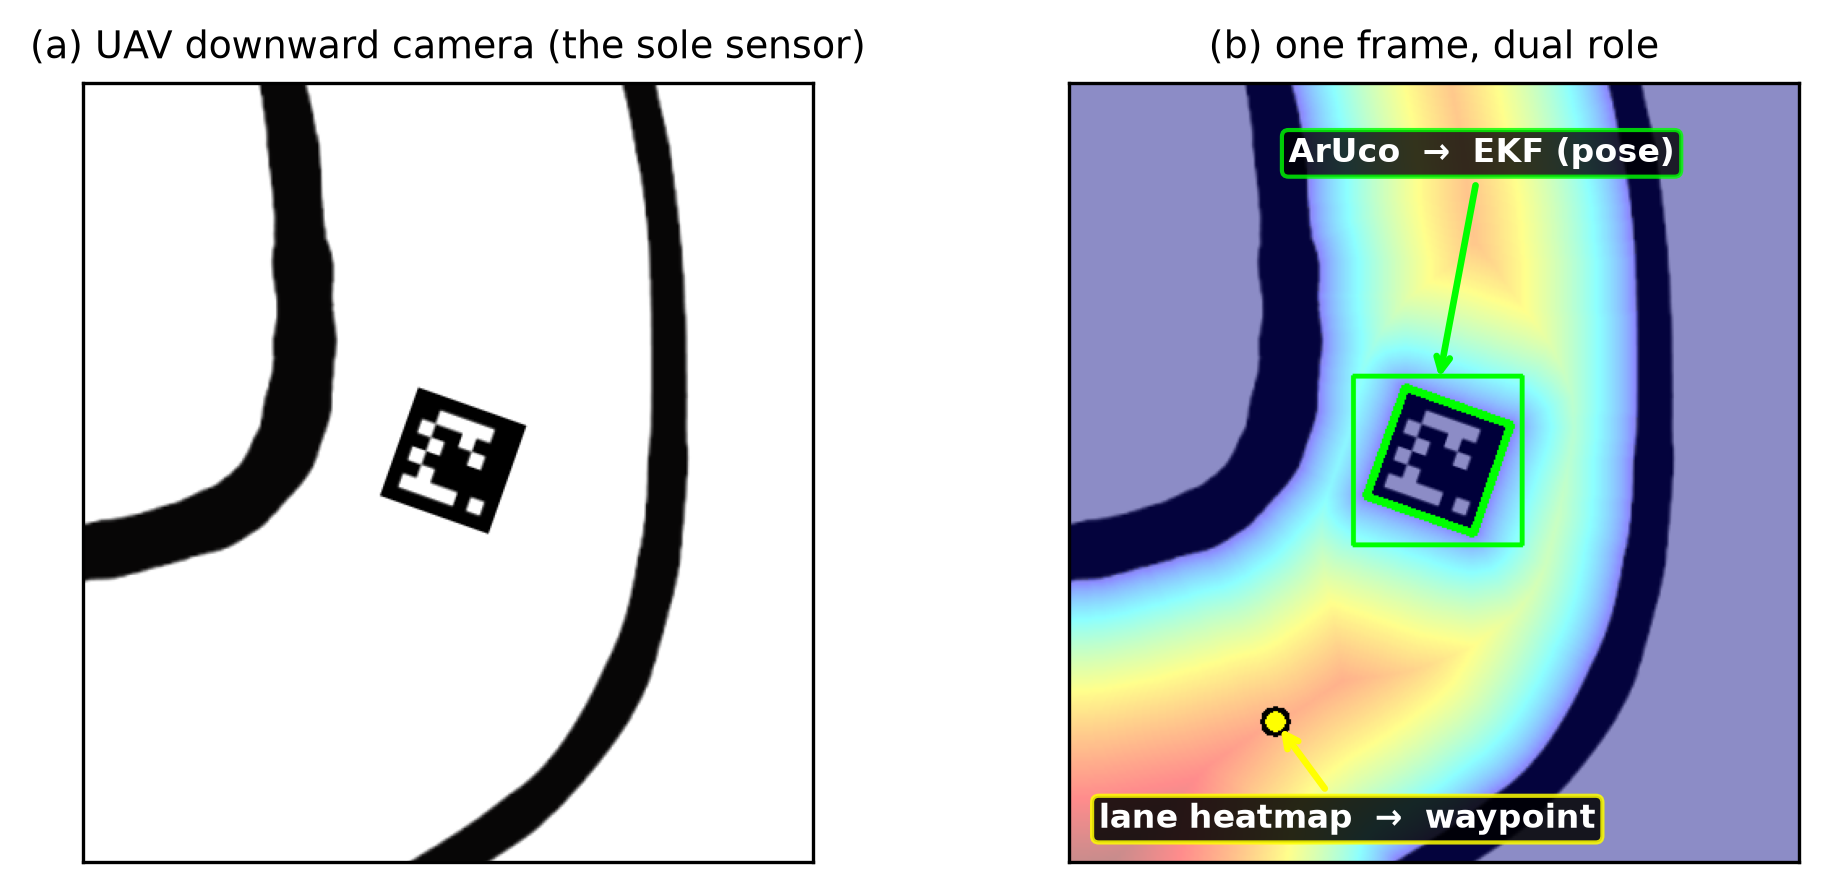
\includegraphics[width=0.99\columnwidth]{media/Fig_Testbed.png}
\caption{The single downward camera in operation (real frame from the headless SITL system).
{(a)} A raw UAV camera image: the curved lane with the UGV's ArUco marker. {(b)} The
{same} frame drives both roles --- the segmented-lane distance-transform heatmap yields the
navigation waypoint (yellow), while the detected ArUco (green) feeds the EKF pose. This is the
shared-sensor coupling the paper studies: one image, two jobs.}
\label{fig:testbed}
\end{figure}

 {Co-design: event-triggering makes the aerial planner affordable.} The belief-space UGV
controller runs continuously --- it is the ground vehicle's feedback loop --- so the compute
lever is the {UAV nominal (aerial) planner} that re-optimizes the aerial tracking trajectory.
Continuous aerial replanning (C1) spends a large, sustained CPU budget; the perception-driven
event trigger (C2) re-solves it only when a covariance/curvature/drift
condition fires. On the nominal track (headless, $R{=}3$), C2 reduces aerial-planner invocations
$\approx\!\RESsolveRed\times$ ($\RESsolvesCone\!\to\!\RESsolvesCthree$) and its CPU
$\approx\!\REScpuRed\times$ ($\REScpuCone\!\to\!\REScpuCthree$\,ms per $45$\,s run;
Table~\ref{tab:results}), at matched estimation quality (steady-state $\tr\Sigma=\REScov$ and
$\approx\!99.9\%$ ArUco visibility for both). Per-solve time is slightly higher for C2 ($\RESmsCthree$
vs.\ $\RESmsCone$\,ms, a warm-start effect), but the $\approx\!\RESsolveRed\times$ reduction in
solve count contributes towards net computational advantages. This is the co-design point: event-triggering makes
perception-aware aerial replanning affordable on a constrained companion computer at estimation
quality indistinguishable from continuous replanning. The one cost is a small loss of
inter-trigger smoothness --- applying the previous nominal between triggers raises high-frequency
trajectory content --- a favorable tradeoff. Isolating how much the {perception-specific}
trigger conditions add beyond a plain error-triggered baseline is a focused ablation for
follow-on work.

\begin{table}[h]
\caption{Aerial-planner co-design (headless, track2, mean\,$\pm$\,std, $R{=}3$). C1 continuous
vs.\ C2 event-triggered; the belief-space UGV controller runs continuously in both.
Steady-state $t\!\ge\!8$\,s.}
\label{tab:results}
\begin{center}
\footnotesize
\setlength{\tabcolsep}{3pt}
\begin{tabular}{|l|c|c|}
\hline
 {Metric} &  {C1 (cont.)} &  {C2 (event)}\\
\hline
Aerial solves (\#/run) & \RESsolvesCone & \RESsolvesCthree\\
\hline
Mean solve (ms) & \RESmsCone & \RESmsCthree\\
\hline
Aerial CPU (ms/run) & \REScpuCone & \REScpuCthree\\
\hline
Steady-state $\tr\Sigma$ & \REScov & \REScov\\
\hline
ArUco vis.\ (\%) & 99.8 & 99.9\\
\hline
UAV--UGV offset (m) & \RESoffCone & \RESoffCthree\\
\hline
\end{tabular}
\end{center}
\end{table}

 {The coverage--resolution altitude tension.} With the GSD model enabled, we sweep
altitude across three tracks of increasing curvature (headless; low-altitude cells are the
median of $R{=}3$ reps). Two costs move oppositely with altitude (Fig.~\ref{fig:envelope}):
estimation uncertainty $\tr\Sigma$ {decreases} as altitude decreases ($0.0094$ at
$z{=}6$\,m to $0.0053$ at $z{=}2$\,m --- the $R\propto z^2$ resolution gain, and
track-independent), while the UGV steering effort needed to keep the path segmented
{increases} as altitude decreases, and increases with path curvature. This is the tension
the altitude policy must resolve: fly as low as segmentation allows, and climb where the
navigation floor rises.

We close the loop with the
perception-constrained policy and compare it against the two natural fixed-altitude baselines on
the hairpin (the most demanding track; headless, GSD noise, $R{=}3$). The policy actuates
altitude over $[\RESaltLo,\RESaltHiZ]$\,m --- holding near the low-altitude floor on straights
and climbing through turns (Fig.~\ref{fig:altpolicy}) --- and it is {not} matched by any
static choice (Fig.~\ref{fig:altpolicy}). The  {fixed-low} baseline ($z{=}2.5$\,m) obtains
good average resolution but suffers coverage-loss transients: as the target leaves the small
footprint in the hairpin, its peak covariance spikes to $\RESaltLowMax$ ($\RESaltLowRatio\times$
the adaptive policy's peak of $\RESaltAdaptMax$) and it drops marker visibility. The
 {fixed-high} baseline ($z{=}7$\,m) never loses coverage but pays a $\RESaltHiPen\%$
estimation penalty ($\tr\Sigma=\RESaltHiMean$ vs.\ $\RESaltAdaptMean$) from the degraded GSD.
The  {adaptive} policy attains the low mean covariance of flying low ($\RESaltAdaptMean$,
matching the fixed-low $\RESaltLowMean$) while keeping the peak covariance and FoV exits of
flying high, demonstrating a favorable balance between estimation accuracy and coverage.
\begin{table}[htbp]
\caption{System Parameters and Controller Hyperparameters\textsuperscript{*}}
\label{tab:system_parameters}
\centering
\begin{tabular}{@{}llc@{}}
\toprule
\textbf{Subsystem} & \textbf{Parameter} & \textbf{Value} \\ 
\midrule
\multirow{3}{*}{Camera / EKF} & Camera FoV ($\phi$) & 1.047 rad \\
 & Baseline Altitude ($z_0$) & 3.0 m \\
 & Baseline Covariance ($R_0$) & $2.5 \times 10^{-3} \text{ m}^2$ \\
 & EKF Update Rate & 20 Hz \\ 
\midrule
\multirow{4}{*}{UGV NMPC} & Horizon ($N$), Step ($dt$) & 5, 0.2 s \\
 & Cost Weights ($Q/R/w_{fov}$) & 10 / 10 / 5 \\
 & Covariance Penalty ($\lambda$) & 1.0 \\
 & Bounds ($v_{max}$, $\omega_{max}$) & 0.22 m/s, 2.0 rad/s \\ 
\midrule
\multirow{4}{*}{UAV Planner} & Horizon ($N$), Step ($dt$) & 10, 0.2 s \\
 & Velocity Bounds ($v_x, v_y, v_z$) & $\pm 1.5, \pm 1.5, \pm 1.0$ m/s \\
 & Altitude Weight ($w_{alt}$) & 50 \\
 & Policy ($z_m$, $\beta_\kappa$) & 0.4 m, 5.0 \\ 
\midrule
\multirow{3}{*}{Tube \& Triggers} & Shape Matrix ($P_0$) & $0.186 I_3$ \\
 & Adaptive Tube Radius ($\alpha$) & $[0.5, 2.0]$ \\
 & Cov. Triggers (spike, drift) & 0.12, 0.07 \\
 & Timing ($T_{min}$, lockout) & 3.0 s, 1.0 s \\ 
\bottomrule
\multicolumn{3}{@{}p{\columnwidth}@{}}{
\footnotesize{\textsuperscript{*} \textbf{Note on Experimental Configurations:} The co-design validation (C1/C2) utilized a fixed reference altitude of $z_{opt} = 6.0$ m to isolate computational metrics. The adaptive altitude policy experiments dynamically actuated altitude within the bounded operational band of $[2.5, 7.0]$ m.}
}
\end{tabular}
\end{table}


\begin{figure}[thpb]
\centering
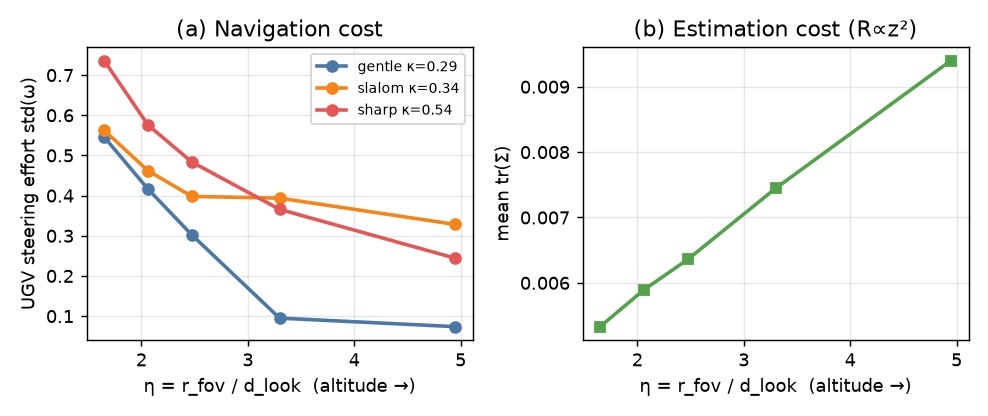
\includegraphics[width=0.78\columnwidth]{media/Fig_Envelope.png}
\caption{The two jaws of the altitude tension ($\eta=r_{\mathrm{fov}}/d_{\mathrm{look}}$,
increasing with altitude). {Left:} UGV steering effort (navigation cost) rises at low
altitude and with path curvature. {Right:} estimation uncertainty $\tr\Sigma$ falls at low
altitude (GSD, $R\propto z^2$; track-independent). The optimum flies as low as segmentation
allows.}
\label{fig:envelope}
\end{figure}

\begin{figure}[t]
\centering
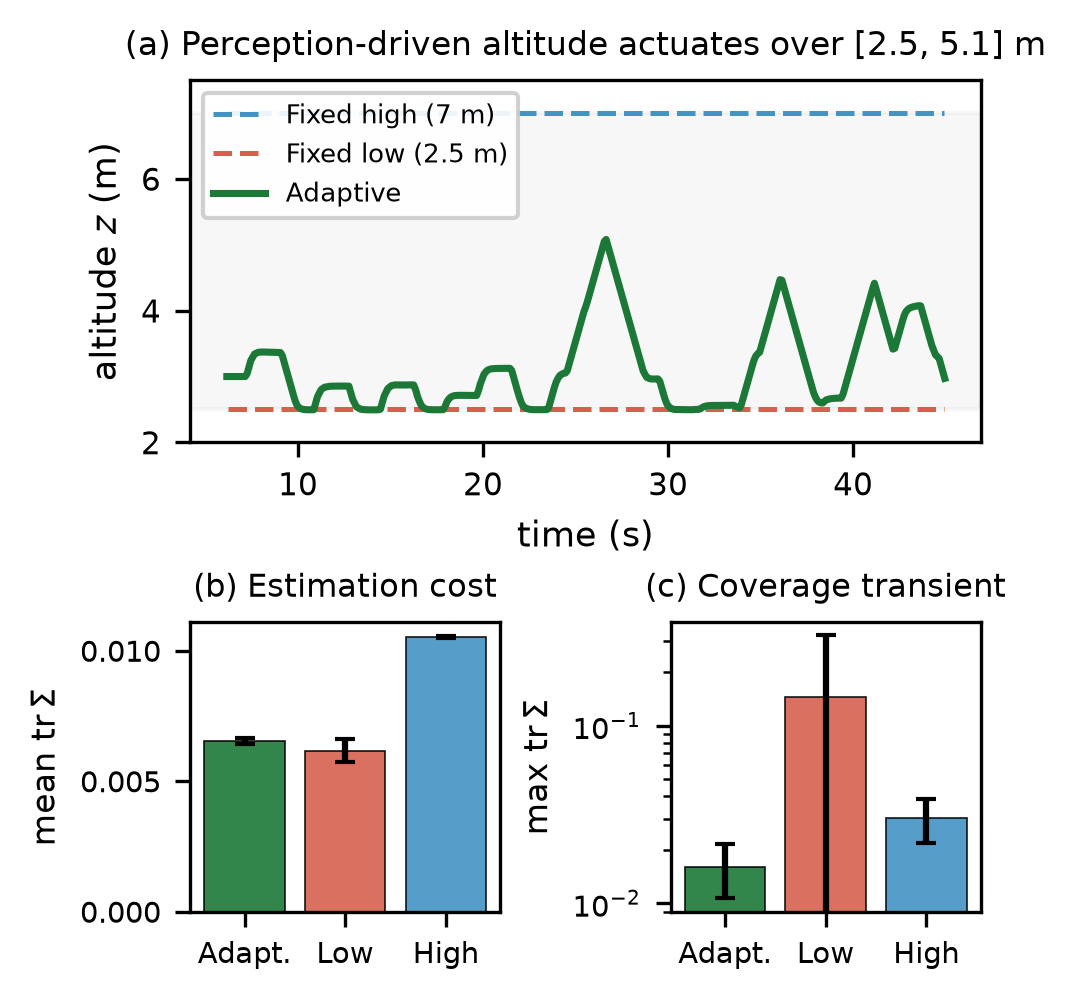
\includegraphics[width=0.80\columnwidth]{media/Fig_AltPolicy.png}
\caption{Adaptive altitude outperforms fixed altitude (hairpin, headless, GSD noise, $R{=}3$).
{(a)} The policy actuates altitude over $[\RESaltLo,\RESaltHiZ]$\,m, holding near the
low-altitude floor on straights and climbing through turns, versus the two static baselines.
{(b)} A fixed-high policy pays a $\RESaltHiPen\%$ mean-estimation penalty. {(c)} A
fixed-low policy suffers coverage-loss transients ($\RESaltLowRatio\times$ larger peak
$\tr\Sigma$, log scale). The adaptive policy achieves a favorable balance between estimation accuracy and coverage.}
\label{fig:altpolicy}
\end{figure}

Consistent with the shared-camera architecture, the estimation uncertainty $\tr\Sigma$ at a given
altitude is largely determined by the measurement noise model and is therefore nearly
track-independent. In contrast, the navigation cost depends strongly on path geometry, so altitude
must balance estimation quality against sufficient camera coverage. At the most demanding operating
point ($z=2$\,m, UGV speed $1.0$\,m/s), occasional simulator timing variations lead to small
run-to-run differences in marker visibility. Rather than identifying a sharp feasibility boundary,
we therefore characterize the tradeoff through the overall performance trends and the comparison
between adaptive and fixed-altitude policies.

\section{CONCLUSIONS}
We studied aerial--ground cooperative tracking where a single downward UAV camera is the ground
vehicle's sole exteroceptive sensor, serving both its navigation reference and its state
estimate. We identified the coverage--resolution altitude tension intrinsic to this shared-sensor
architecture and demonstrated closed-loop that the perception-constrained altitude policy
resolving it achieves lower peak estimation error than the low-altitude baseline ($\RESaltLowRatio\times$ smaller peak covariance) while avoiding the sustained estimation penalty of the high-altitude baseline ($\RESaltHiPen\%$ estimation penalty) 

We further showed a perception-driven event trigger
cuts the UAV nominal (aerial) planner's re-solves $\approx\!\RESsolveRed\times$ and its CPU
$\approx\!\REScpuRed\times$ at matched estimation quality, and we release the
reproducible testbed. Future work: a full multicopter model for hardware-faithful altitude
dynamics; a second exteroceptive sensor to isolate the observability benefit; and a homothetic
tube carrying recursive-feasibility guarantees into the online loop.

\subsection{Limitations and Future Work}

The present study is limited to software-in-the-loop evaluation using a velocity-controlled UAV abstraction and a single-camera sensing architecture. While the proposed controller is motivated by an offline robust-MPC design, the implemented online controller employs a computationally efficient ellipsoidal surrogate rather than a full tube-MPC formulation. Consequently, the results should be interpreted as an empirical evaluation of the proposed perception-aware architecture under controlled simulation conditions.

Future work will extend the framework to hardware experiments with a full multicopter model, investigate stronger theoretical guarantees for the adaptive online controller, compare against additional event-trigger formulations, and evaluate the approach under more challenging perception conditions including intermittent observations, latency, and occlusions.

%%%%%%%%%%%%%%%%%%%%%%%%%%%%%%%%%%%%%%%%%%%%%%%%%%%%%%%%%%%%%%%%%%%%%%%%%%%%%%%%

\begin{thebibliography}{99}

\bibitem{mayne2005robust} D. Q. Mayne, M. M. Seron, and S. V. Rakovi\'c,
``Robust model predictive control of constrained linear systems with bounded
disturbances,'' {Automatica}, vol.~41, no.~2, pp.~219--224, 2005.

\bibitem{mRPI} S. V. Rakovic, E. C. Kerrigan, K. I. Kouramas, and D. Q. Mayne,
``Invariant approximations of the minimal robust positively invariant set,''
{IEEE Trans. Autom. Control}, vol.~50, no.~3, pp.~406--410, 2005.

\bibitem{mayne2000constrained} D. Q. Mayne, J. B. Rawlings, C. V. Rao, and
P. O. M. Scokaert, ``Constrained model predictive control: Stability and
optimality,'' {Automatica}, vol.~36, no.~6, pp.~789--814, 2000.

\bibitem{falanga2018pampc} D. Falanga, P. Foehn, P. Lu, and D. Scaramuzza,
``PAMPC: Perception-aware model predictive control for quadrotors,'' in
{IEEE/RSJ Int. Conf. Intelligent Robots and Systems (IROS)}, 2018.

\bibitem{platt2010belief} R. Platt, R. Tedrake, L. Kaelbling, and
T. Lozano-P\'erez, ``Belief space planning assuming maximum likelihood
observations,'' in {Robotics: Science and Systems (RSS)}, 2010.

\bibitem{vandenberg2012motion} J. van den Berg, S. Patil, and R. Alterovitz,
``Motion planning under uncertainty using iterative local optimization in belief
space,'' {Int. J. Robotics Research}, vol.~31, no.~11, pp.~1263--1278, 2012.

\bibitem{eqtami2010event} A. Eqtami, D. V. Dimarogonas, and K. J. Kyriakopoulos,
``Event-triggered control for discrete-time systems,'' in {American Control
Conference (ACC)}, 2010, pp.~4719--4724.

\bibitem{langson2004tubes} W. Langson, I. Chryssochoos, S. V. Rakovi\'c, and D. Q. Mayne,
``Robust model predictive control using tubes,'' {Automatica}, vol.~40, no.~1,
pp.~125--133, 2004.

\bibitem{mayne2011tube} D. Q. Mayne, E. C. Kerrigan, E. J. van Wyk, and P. Falugi,
``Tube-based robust nonlinear model predictive control,'' {Int. J. Robust Nonlinear
Control}, vol.~21, no.~11, pp.~1341--1353, 2011.

\bibitem{chisci2001persistent} L. Chisci, J. A. Rossiter, and G. Zappa, ``Systems with
persistent disturbances: Predictive control with restricted constraints,'' {Automatica},
vol.~37, no.~7, pp.~1019--1028, 2001.

\bibitem{heemels2012introduction} W. P. M. H. Heemels, K. H. Johansson, and P. Tabuada,
``An introduction to event-triggered and self-triggered control,'' in {IEEE Conf.
Decision and Control (CDC)}, 2012, pp.~3270--3285.

\bibitem{tabuada2007event} P. Tabuada, ``Event-triggered real-time scheduling of stabilizing
control tasks,'' {IEEE Trans. Autom. Control}, vol.~52, no.~9, pp.~1680--1685, 2007.

\bibitem{li2014event} H. Li and Y. Shi, ``Event-triggered robust model predictive control of
continuous-time nonlinear systems,'' {Automatica}, vol.~50, no.~5, pp.~1507--1513, 2014.

\bibitem{spasojevic2020perception} I. Spasojevic, V. Murali, and S. Karaman,
``Perception-aware time optimal path parameterization for quadrotors,'' in {IEEE Int.
Conf. Robotics and Automation (ICRA)}, 2020, pp.~3213--3219.

\bibitem{zhang2019fisher} Z. Zhang and D. Scaramuzza, ``Beyond point clouds: Fisher information
field for active visual localization,'' in {IEEE Int. Conf. Robotics and Automation
(ICRA)}, 2019, pp.~5986--5992.

\bibitem{prentice2009belief} S. Prentice and N. Roy, ``The belief roadmap: Efficient planning
in belief space by factoring the covariance,'' {Int. J. Robotics Research}, vol.~28,
no.~11--12, pp.~1448--1465, 2009.

\bibitem{kaelbling1998planning} L. P. Kaelbling, M. L. Littman, and A. R. Cassandra,
``Planning and acting in partially observable stochastic domains,'' {Artificial
Intelligence}, vol.~101, no.~1--2, pp.~99--134, 1998.

\bibitem{indelman2015planning} V. Indelman, L. Carlone, and F. Dellaert, ``Planning in the
continuous domain: A generalized belief space approach for autonomous navigation in unknown
environments,'' {Int. J. Robotics Research}, vol.~34, no.~7, pp.~849--882, 2015.

\bibitem{placed2023survey} J. A. Placed, J. Strader, H. Carrillo, N. Atanasov, V. Indelman,
L. Carlone, and J. A. Castellanos, ``A survey on active simultaneous localization and mapping:
State of the art and new frontiers,'' {IEEE Trans. Robotics}, vol.~39, no.~3,
pp.~1686--1705, 2023.

\bibitem{cadena2016past} C. Cadena, L. Carlone, H. Carrillo, Y. Latif, D. Scaramuzza, J. Neira,
I. Reid, and J. J. Leonard, ``Past, present, and future of simultaneous localization and
mapping: Toward the robust-perception age,'' {IEEE Trans. Robotics}, vol.~32, no.~6,
pp.~1309--1332, 2016.

\bibitem{li2024colag} Z. Li, R. Mao, N. Chen, C. Xu, F. Gao, and Y. Cao, ``ColAG: A
collaborative air-ground framework for perception-limited UGVs' navigation,'' in {IEEE
Int. Conf. Robotics and Automation (ICRA)}, 2024, pp.~16781--16787.

\bibitem{santos2024aerial} M. Ferreira Santos, P. Castillo, and A. Corr\^ea Victorino,
``Aerial vision based guidance and control for perception-less ground vehicle,'' in
{European Control Conference (ECC)}, 2024, pp.~2780--2785.

\bibitem{grocholsky2006cooperative} B. Grocholsky, J. Keller, V. Kumar, and G. Pappas,
``Cooperative air and ground surveillance,'' {IEEE Robotics Autom. Mag.}, vol.~13, no.~3,
pp.~16--25, 2006.

\bibitem{thomas2017autonomous} J. Thomas, J. Welde, G. Loianno, K. Daniilidis, and V. Kumar,
``Autonomous flight for detection, localization, and tracking of moving targets with a small
quadrotor,'' {IEEE Robotics Autom. Lett.}, vol.~2, no.~3, pp.~1762--1769, 2017.

\bibitem{penin2018vision} B. Penin, P. Robuffo Giordano, and F. Chaumette, ``Vision-based
reactive planning for aggressive target tracking while avoiding collisions and occlusions,''
{IEEE Robotics Autom. Lett.}, vol.~3, no.~4, pp.~3725--3732, 2018.

\bibitem{roumeliotis2002distributed} S. I. Roumeliotis and G. A. Bekey, ``Distributed
multirobot localization,'' {IEEE Trans. Robotics Autom.}, vol.~18, no.~5, pp.~781--795,
2002.

\bibitem{kia2016cooperative} S. S. Kia, S. Rounds, and S. Mart\'inez, ``Cooperative
localization for mobile agents: A recursive decentralized algorithm based on Kalman-filter
decoupling,'' {IEEE Control Syst. Mag.}, vol.~36, no.~2, pp.~86--101, 2016.

\end{thebibliography}


\end{document}
